\documentclass[twocolumn,linenumbers]{aastex631}
\usepackage{physics}
\usepackage{gensymb}

% Operators
\DeclareMathOperator*{\argmax}{arg\,max}
\DeclareMathOperator*{\argmin}{arg\,min}
\DeclareMathOperator*{\diag}{diag}
\newcommand{\exptval}[1]{\mathbb{E}\left[ #1 \right]}
\newcommand{\Var}[1]{\text{Var}\qty[#1]}
\newcommand{\Cov}[1]{\text{Cov}\qty[#1]}

% variables
\newcommand{\bb}[1]{\mathbb{#1}}
\newcommand{\vbd}{\vb{d}}
\newcommand{\vbm}{\vb{m}}
\newcommand{\vbep}{\vb{\varepsilon}}
\newcommand{\vbn}{\vb{n}}
\newcommand{\vbb}{\vb{b}}
\newcommand{\inv}[1]{#1^{-1}}
\newcommand{\noisevar}{\Sigma_{\vbn}}
\newcommand{\hatm}{\vb{\hat{m}}}
\newcommand{\Pdagger}{P^{\dagger}}
\newcommand{\Nbar}{\bar{N}}
\newcommand{\PPinv}[1]{\inv{\qty(\Pdagger #1 P)}}
\newcommand{\Neta}{N_{\eta}}

\newcommand{\kmh}[1]{\textcolor{red}{KMH: #1}}


%\submitjournal{ApJ}
\graphicspath{{./}{figures/}}

\begin{document}

\title{Perturbative Approach to Solve the Map-Making Equation}

\footnote{
The source code and other information are available at \url{https://github.com/Bai-Qiang/map_making_perturbative_approach}
}

\author{Bai-Qiang Qiang}
\affiliation{Department of Physics, Florida State University, Tallahassee, Florida 32306}

\author[0000-0001-7109-0099]{Kevin M. Huffenberger}
\affiliation{Department of Physics, Florida State University, Tallahassee, Florida 32306}


\begin{abstract}
  \kmh{I think we need a new title.  Perturbation usually means a small change, whereas this is a big change that we apply gradually. Word ideas: ``Linear system, map-making, Cosmic Microwave Background, annealing,''}

In the context of the Cosmic Microwave Background, we study the solution to the equation that transforms scanning data into a map.  We show that splitting the noise covariance into two parts, as suggested by ``messenger'' methods for solving linear systems, is particularly effective when there is significant low-frequency noise in the timestream.  A conjugate gradient algorithm applied to the modified system converges faster and to a higher fidelity solution than the standard approach, for the same computational cost per iteration.
%We present a method to solve map-making equation by reinterpret messenger field method and using conjugate gradient algorithm.
%We separating noise covariance matrix $N$ into two parts, white noise part and the remaining noise part as perturbation, with perturbation parameter $\eta$.
%
We give an analytical expression for the parameter that controls how gradually the non-uniform noise is switched on during the course of the solution. 

\end{abstract}

%% Keywords should appear after the \end{abstract} command. 
%% The AAS Journals now uses Unified Astronomy Thesaurus concepts:
%% https://astrothesaurus.org
%% You will be asked to selected these concepts during the submission process
%% but this old "keyword" functionality is maintained in case authors want
%% to include these concepts in their preprints.
%\keywords{Classical Novae (251) --- Ultraviolet astronomy(1736) --- History of astronomy(1868) --- Interdisciplinary astronomy(804)}
\keywords{Some Keywords}

%% From the front matter, we move on to the body of the paper.
%% Sections are demarcated by \section and \subsection, respectively.
%% Observe the use of the LaTeX \label
%% command after the \subsection to give a symbolic KEY to the
%% subsection for cross-referencing in a \ref command.
%% You can use LaTeX's \ref and \label commands to keep track of
%% cross-references to sections, equations, tables, and figures.
%% That way, if you change the order of any elements, LaTeX will
%% automatically renumber them.
%%
%% We recommend that authors also use the natbib \citep
%% and \citet commands to identify citations.  The citations are
%% tied to the reference list via symbolic KEYs. The KEY corresponds
%% to the KEY in the \bibitem in the reference list below. 

\section{Introduction} \label{sec:intro}

%The cosmic microwave background is an electromagnetic radiation coming from early
%stage of our Universe. Based on the hot Big Bang model, before the recombination
%epoch, the photons were tightly coupled with free electrons and protons via 
%Thomson scattering. As the universe expanded and cooled down, free electrons and
%protons combined into neutral hydrogen atom.  This process is called 
%recombination in cosmology. Shortly after this epoch, the photons could
%propagate freely and would not be scattered by charged particles. Today, we receive
%the photons produced at that time and called them the cosmic microwave background
%radiation. Studying these photons coming from early universe can help us
%to constrain theoretical model and cosmological parameters
%\cite{10.1093/ptep/ptaa104}.
%The next generation CMB observations will have much higher resolution and 
%generate more data. So we need an efficient way to process the data.
%One step of the the processing is map making, which gives an estimated map based on the raw observation data.

%map-making
Map-making is an intermediate process between data collection and estimate
various cosmological parameters.
As the next generation CMB observations will have much higher resolution and 
generate more data, we need an efficient way to process the data.
There are many map-making methods introduced in \cite{1997ApJ...480L..87T}.
Currently, one the most commonly used method is COBE method.

Recently \cite{2013A&A...549A.111E} introduced a new
method called messenger field to solve Wiener filter,
and then this technique was being applied to map-making by
\cite{Huffenberger_2018},
and messenger field could outperform traditional conjugate gradient method, 
with proper cooling technique.
It has been shown by \cite{2018A&A...620A..59P} this messenger field method
is equivalent to applying a preconditioner to the original problem and 
introducing an extra cooling parameter $\lambda$,
but whether this cooling parameter will boost performance compare to
 the (traditional) conjugate gradient method is still controversial . 
Here I give a detailed analysis of this parameter and show that
it may improve performance under some circumstances, if we properly choose
its values.


The map making procedure could be summarized in equation
\begin{equation}
\vbd = P\vbm + \vbn \label{map making model}
\end{equation}
where $\vbd$, $P$, $\vbm$, $\vbn$ are time-ordered data (TOD), pointing matrix,
CMB map, and noise.
%The time-ordered data we collected is given by map signal $P\vbm$ plus noise 
%$\vbn$.
%The pointing matrix $P$ acting on the map gives the signal of the map at some specific 
%position of sky where telescope is pointing at.
Here we assume that the noise has zero mean $\ev{\vbn} = \vb{0}$,
and noise covariance matrix could be written as $N = \ev{\vbn \vbn^{\dagger}}$.

As we can see the map making model Eq.(\ref{map making model}) mathematically 
is a standard linear regression problem,
with \textit{design matrix} being pointing matrix $P$, and \textit{regression
coefficients} are $\vbm$.
For COBE method, we estimate linear regression coefficients $\vbm$ with
\textit{generalized least square} (GLS) technique, since the noise $\vbn$ is 
\textit{heteroscedastic}.
%: the variances $N$ are different for various frequencies.
%Usually detectors have a $1/f$ noise pattern
%\cite{1997PhRvD..56.4514T}.
%The \textit{generalized least square} (GLS) will provide better estimation 
%than \textit{ordinary least square} (OLS) method, because the data is
%heteroscedastic so we would like to focusing on fitting the data with lower 
%noise.
%then the estimated map $\hatm$ minimize
The GLS minimize
\begin{align}
\chi^2(\vbm) & \equiv (\vbd - P\vbm)^{\dagger} N^{-1} (\vbd - P \vbm).
\label{chi2 formula}
\end{align}
and the estimated map $\hatm$ is given by
\begin{equation}
\hatm = \argmin_{\vbm}  \chi^2(\vbm) = \PPinv{N} \Pdagger \inv{N} \vbd 
\end{equation}
Or rewrite it as 
\begin{align}
\qty(\Pdagger \inv{N}  P) \hatm = \Pdagger \inv{N} \vbd \label{map making eq}
\end{align}
This is the map-making equation we need to solve.
However, based on current computation power, it is impossible to solve $\hatm$
by calculating $\PPinv{\inv{N}} \Pdagger \inv{N} \vbd$ directly,
since the noise covariance matrix $N$ is sparse in frequency domain,
and pointing matrix $P$ is sparse in (time by pixel) domain.
In experiments currently under design, there may be $\sim 10^{16}$ time samples
and $\sim 10^{9}$ pixels, so these matrix inversions are intractable.
%It is impossible to do these matrix multiplication directly and then take
%inverse.
Therefore we use Conjugate Gradient method, which is an iterative algorithm,
to solve this map-making equation.
For simplicity we fix the preconditioner being $M= \Pdagger P$ for all of 
calculations.

The structure of this paper is organized as follows.
In section 2 we briefly introduce messenger field fixed point iteration method
and preconditioned version.
In section 3 we reinterpret this process and give an analysis on how to determine
the parameters.
Section 4 gives the noise power spectrum in our simulation, and Section 5 shows
results.
Finally, Section 6 we discuss this method's pro and con for possible future 
improvements.


\section{Messenger Field Method}

Messenger field method separate noise covariance matrix
$N = \Nbar + T$, with $T = \tau I $ and $\tau$ being the minimum eigenvalue of
$N$.
Then there is a cooling parameter $\lambda$ such that 
$N(\lambda) = \Nbar + \lambda T$, with initial $\lambda$ being a very large
number and final $\lambda$ being $1$.

After apply preconditioner $\Pdagger \inv{T} P$ to the map making equation
Eq.(\ref{map making eq}), we would get:
\begin{align}
\begin{aligned}[b]
\hatm &= \PPinv{\inv{T}} \Pdagger \inv{T} 
    \inv{\qty(\inv{T} + \inv{\Nbar})} 
\\ &\mathrel{\phantom{=}} \quad \times \qty[ \inv{T}P\hatm + \inv{\Nbar}\vbd]
\end{aligned}
\end{align}

To add cooling parameter $\lambda$, we need to change $T$ to $\lambda T$
and $N$ to $N(\lambda)$.
Then we could  rewrite it as a fixed point iteration form
\begin{equation}
\left\{\!
\begin{aligned}
\vb{t}_i &= \inv{\qty(\inv{(\lambda T)} + \inv{\Nbar})} 
    \qty[ \inv{(\lambda T)}P\hatm_i + \inv{\Nbar}\vbd]\\
\hatm_{i+1} &= \PPinv{\inv{(\lambda T)}} \Pdagger \inv{(\lambda T)} \vb{t}_i 
\end{aligned}
\right.
\end{equation}
This is fixed point iteration form of messenger field method.
It's equivalent to solving map-making equation Eq.(\ref{map making eq}) with
preconditioner $\Pdagger \inv{(\lambda T)} P = \inv{\tau} \Pdagger P$.
This preconditioner is equivalent to preconditioner $M = \Pdagger P$,
since multiply a constant won't change condition number.
Therefore messenger field is solving modified map making equation
\begin{align}
\Pdagger \inv{N(\lambda)}  P\ \hatm = \Pdagger \inv{N(\lambda)} \vbd
\end{align}
with preconditioner $M = \Pdagger P$.
More detailed derivation could be found in \cite{2018A&A...620A..59P}.


%\begin{align}
%\PPinv{\inv{(\lambda T)}} \Pdagger \inv{(\Nbar + \lambda T)} P \hatm
%= \PPinv{\inv{(\lambda T)}} \Pdagger \inv{(\Nbar + \lambda T)} \vbd
%\end{align}

%If we substitute $T = \tau I$, then messenger field method is equivalent solving
%If we add 
%\begin{align}
%\begin{aligned}[b]
%&\PPinv{} \Pdagger \inv{\qty(\tau I + \frac{1}{\lambda}\Nbar)} P \hatm 
%\\&\quad= \PPinv{} \Pdagger \inv{\qty(\tau I + \frac{1}{\lambda}\Nbar)} \vbd
%\end{aligned}
%\label{lambda eta equiv}
%\end{align}
%since multiplying a constant won't change the condition number, it's equivalent
%to solve map making equation with perturbation parameter $\eta = 1/\lambda$ and
%simple preconditioner.

%The map making equation Eq.(\ref{map making equation}) derived from Generalized
%Least Square estimation,
%Rewrite the map making equation Eq.(\ref{map making equation}) in the form
%\begin{align}
%\qty(\Pdagger \inv{N}  P) \hatm = \Pdagger \inv{N} \vbd \label{map making eq}
%\end{align}
%If we define $A = \Pdagger \inv{N} P$ and $\vbb = \Pdagger \inv{N} \vbd$,
%then it could be written as $A\hatm = \vbb$.

%However, for a vector with size of map $\hatm$, we could calculate
%$\Pdagger \inv{N} P \hatm = A\hatm$ by first taking Fourier transform $P\hatm$
%then inverse Fourier transform $\inv{N}P\hatm$.
%This means it can be solved by the conjugate gradient method.


%\subsection{Preconditioner}
%To improve the performance of the conjugate gradient method,
%we could apply a preconditioner $M$ to original problem $A\hatm = \vbb$,
%which then becomes $\inv{M}A\hatm = \inv{M} \vbb$.
%The preconditioner should reduce the condition number of original problem,
%so that the conjugate gradient method will converge faster.
%We want the preconditioner to capture as much information as possible from 
%matrix $A$, but still keep it relative easy to calculate $\inv{M}$.
%For example, if $M = A$, $\inv{M} A \hatm = \inv{M} \vbb$ would be solved
%immediately, but $\inv{M}$ will be extremely difficult to calculate.
%We could simply choose $M = \Pdagger P$,
%and the operation $\inv{M} \vbm = \PPinv{} \vbm$ is the average over each pixel 
%of map $\vbm$.
%
%For the conjugate gradient method, we need an initial guess map $\hatm_0$. 
%We can use zero vector $\hatm_0 = \vb{0}$ as initial guess,
%but the simple binned map $\hatm_0 = \PPinv{} \Pdagger \vbd$ is a better 
%choice (it is a the solution for white noise case $N \propto I$).
%(Pape\v{z} et al. 2018\cite{2018A&A...620A..59P}) showed that using 
%$\hatm_0$ as initial guess could improve performance significantly compare to
%zero vector $\vb{0}$ in come cases.
%As stated before, we can calculate $\PPinv{}$ acting on any map-sized object,
%and $\Pdagger \vbd$ is indeed a map size object, 
%so we could obtain simple binned map by calculating
%$\hatm_0 = \PPinv{} \Pdagger \vbd$ directly.
%
%For the conjugate gradient method with simple preconditioner $M = \Pdagger P$,
%we have all we need.  Next we only need to use conjugate gradient algorithm solve the problem.

\section{Parameterized Conjugate Gradient Method}

\subsection{Introduce the Idea}
The messenger field method introduced an extra cooling parameter $\lambda$ to
map-making equation, so we want to know how to choose this parameter.
In \cite{2017MNRAS.468.1782K}, they showed that for Wiener filter the cooling
parameter should be chosen as a geometric series.
In this work, we are going to give an alternative interpretation of the
parameterizing process then show that for map-making equation the optimal choice
for $\lambda$ would also be a geometric series.

Based on previous analysis, we know that what messenger field method really
does is parameterizing the map-making equation.
Here to avoid confusion, we introduce another parameter $\eta$, such that the 
parameterized map-making equation is
\begin{align}
\Pdagger \inv{N(\eta)}  P\ \hatm = \Pdagger \inv{N(\eta)} \vbd
\label{map making eq eta}
\end{align}

%Here we now show that we can improve performance in some cases by using a parameterized version of the map making equation Eq.(\ref{map making eq}).
The idea is that map-making equation Eq.(\ref{map making eq}) is hard to solve
due to noise covariance matrix is sandwiched between $\Pdagger P$.
But if noise covariance matrix $N$ is proportional to identity matrix $I$, 
then its solution is given by simple binned map
$\vbm_0 = \inv{\qty(\Pdagger P)} \Pdagger \vbd$,
which could be solved directly. 
We can parameterize the noise covariance matrix $N$ with a parameter $\eta$,
such that initially $\eta = \eta_i$ we have $N\qty(\eta_i) \propto I$.
In the end $\eta = \eta_f$ and $N\qty(\eta_f) \propto N$,
such that the final solution is what we want.
We expect that the parameterized noise covariance matrix $N(\eta)$
would connect our initial guess $\hatm_0$ and final solution $\hatm$ as we 
change $\eta$ from $\eta_i$ to $\eta_f$, such that it would help improve
convergence speed.

%Now instead of Eq.(\ref{map making eq}), we are solving
%\begin{align}
%\qty(\Pdagger \inv{N(\eta)} P)\, \hatm(\eta) 
%= \Pdagger \inv{N(\eta)} \vbd \label{map making para}
%\end{align}

Now question is how to find $N(\eta)$ such that $N(\eta_i) \propto I$
and $N (\eta_f) \propto N$?
Since the non-white noise part of $N$ is the difficult portion,
we could think of it as a perturbation term, which adds upon the white noise.
Initially there is only white noise and solution is given by $\hatm_0$,
then we gradually add extra noise into this equation by changing $\eta$ from 
$0$ to $1$.
At the end when $\eta=1$ we are solving equation Eq.(\ref{map making eq}).

Therefore we separate noise covariance matrix into two parts
$N = \tau I + \Nbar$ where $\tau$ is the minimum eigenvalue of $N$. 
Then we define $N(\eta) = \tau I + \eta \Nbar$, 
with perturbation parameter $\eta$ which satisfies $\eta_i = 0$ and $\eta_f=1$.

Eq.(\ref{map making eq eta}) then becomes
\begin{align}
\qty(\Pdagger \inv{(\tau I + \eta \Nbar)}P) \, \hatm(\eta) 
= \Pdagger \inv{\qty(\tau I + \eta \Nbar)} \vbd \label{map making perturb} 
\end{align}

We require the perturbation parameter $\eta$ being monotonically increase
series $0 = \eta_0 < \eta_1 < \cdots < \eta_n = 1$.
For some specific $\eta_m$, we use conjugate gradient method to solve equation 
$\qty(\Pdagger \inv{N(\eta_m)} P)\, 
\hatm(\eta_m) = \Pdagger \inv{N(\eta_m)} \vbd$
with simple preconditioner $\Pdagger P$,
and using $\hatm(\eta_{m-1})$ as the initial value.
The initial guess is $\hatm(\eta_0) = \vbm_0 = \PPinv{} \Pdagger \vbd$.

As you can see, $\eta$ is the reciprocal of $\lambda$.
The reason I switch to $\eta$ in stead of keeping $\lambda$ is that it would
be easier for further derivations, and it's a different interpretation.

\subsection{Choosing perturbation parameters $\eta$}
The next question is how we choose these monotonically increasing parameters
$\eta$. 
If we choose these parameters inappropriately, it would only makes it converge
slower.
Also we want to determine $\eta_1, \cdots, \eta_{n-1}$ before starting conjugate
gradient iteration.
That's because time ordered data $\vbd$ is very large,
and we don't want to keep it in the system RAM during calculation.
If $\eta_1, \cdots, \eta_{n-1}$ could be determined before the iterations, 
then we can first calculate $\Pdagger \inv{N(\eta)} \vbd$ for each $\eta_m$
and store these map-sized objects in RAM,
instead of the entire time-ordered data $\vbd$.

First let us try to find out our starting point $\eta_1$.
What would be good value for $\eta_1$?

Here to simplify notation, I will use $\Neta$ to denote $N(\eta)$.
The parameterized estimated map
$\hatm(\eta) = \PPinv{\inv{\Neta}} \Pdagger \inv{\Neta} \vbd$
minimizes the parameterized
\begin{align}
\chi^2 (\vbm, \eta)
= \qty(\vbd - P \vbm)^{\dagger} \inv{\Neta} (\vbd - P\vbm).
\label{chi2 eta formula}
\end{align}
For some specific $\eta$ value, the minimum $\chi^2$ value is given by
\begin{align}
\begin{aligned}[b]
\chi^2 (\hatm(\eta), \eta)
&= \qty\big(\vbd - P \hatm(\eta))^{\dagger} \inv{\Neta} 
    \qty\big(\vbd - P\hatm(\eta))
\end{aligned}
\end{align}
To further simplify the analysis, let's assume that the noise covariance matrix
$N = \ev{\vbn\vbn^{\dagger}}$ is diagonal in the frequency domain.

%Now let us see how $\chi^2(\hatm(\eta),\eta)$ changes as we change $\eta$.
%The relative decrease of $\chi^2(\hatm(\eta), \eta)$ at $\eta$ is defined as
%\begin{align}
%\begin{aligned}[b]
%&-\frac{\delta \chi^2(\hatm(\eta),\eta)} {\chi^2(\hatm(\eta), \eta)}\\
%=& 
%\delta \eta 
%\frac{\qty(\vbd - P\hatm(\eta))^{\dagger}
%    \inv{\Neta} \Nbar \inv{\Neta}
%    (\vbd - P\hatm(\eta)) 
%}
%{\qty\big(\vbd - P \hatm(\eta))^{\dagger} 
%    \inv{\Neta}
%    \qty\big(\vbd - P\hatm(\eta))
%}
%\end{aligned}
%\end{align}
%Here we put a minus sign in front of
%$\delta\chi^2(\hatm(\eta), \eta)/\chi^2(\hatm(\eta), \eta)$,
Let's first consider $\eta_1 = \eta_0 + \delta\eta = \delta\eta$
such that $\eta_1 = \delta \eta$ is very small quantity.
Then the relative decrease of $\chi^2(\hatm(0),0)$ from $\eta_0= 0$ to 
$\eta_1 = \delta \eta$ is
\begin{align}
\begin{aligned}[b]
-\frac{\delta \chi^2(\hatm(0), 0)}{\chi^2(\hatm(0), 0)} 
&= \delta \eta 
\frac{1}{\tau}
\frac{\qty(\vbd - P\hatm(0))^{\dagger} \Nbar  (\vbd - P\hatm(0)) }
    {\qty\big(\vbd - P \hatm(0))^{\dagger} \qty\big(\vbd - P\hatm(0))}
%\\
%& \leq  \frac{\delta \eta}{\tau} \max(\Nbar_f)
\label{eta upper bound}
\end{aligned}
\end{align}
Here we put a minus sign in front of this expression
such that it's non-negative.

%where in first line we used the property $N_{\eta=0} = \tau I$,
%and in second line we used the property that the positive semi-definite $\Nbar$ is diagonal in frequency 
%domain and its maximum eigenvalue is $\max(\Nbar_f)$.
%To prove this, notice that matrix $\Nbar$ is diagonalized in frequency space 
%with eigenvalues $\Nbar_f\geq0$ and the corresponding eigenvectors $\vb{e}_f$
%(these eigenvectors form a complete orthogonal basis).
%Any vector could be decomposed into these frequency basis
%$\vb{v} = \sum_f \alpha_f \vb{e}_f$, therefore we have
%$\frac{\vb{v}^{\dagger} \Nbar \vb{v}}{\vb{v}^{\dagger} \vb{v}} 
%= \frac{\sum_f \alpha_f^2\Nbar_f}{\sum_f \alpha_f^2}
%\leq \max(\Nbar_f) $

Ideally, we want
$\delta \chi^2(\hatm(0),0) = \chi^2(\hatm(1), 1) - \chi^2(\hatm(0),0)$,
such that it would get close to the final $\chi^2$ at next iteration.
Here if we assume that initial $\chi^2$ value $\chi^2(\hatm(0),0)$ is much
larger than final value $\chi^2(\hatm(1),1)$,
then we would expect
$\qty|\delta\chi^2(\hatm(0),0)/\chi^2(\hatm(0),0)| \approx 1^-$,
strictly smaller than 1.
To make sure it will not start too fast, 
we could set its upper bound equal to 1, $\delta \eta \max(\Nbar_f) / \tau = 1$.
This gives
\begin{equation}
\eta_1 = \frac{\tau}{\max(\Nbar_f)} = \frac{\min(N_f)}{\max(N_f) - \min(N_f)}
\end{equation}
Here $N_f$ and $\Nbar_f$ are the eigenvalues of $N$ and $\Nbar$ under frequency
domain.
If the condition number of noise covariance matrix
$\kappa(N) = \max(N_f)/\min(N_f) \gg 1$,
then $\eta_1 \approx \inv{\kappa} (N)$.

What about the other parameters $\eta_m$ with $m > 1$?
We could use a similar analysis,
let $\eta_{m+1} = \eta_m + \delta \eta_m$ with a small $\delta\eta_m$,
and set the upper bound of relative decrease equal to 1.
See Appendix \ref{derive other etas} for detailed derivation.
We would get
%\begin{align}
%\begin{aligned}[b]
%&-\frac{\delta \chi^2(\hatm(\eta_m), \eta_m)}{\chi^2(\hatm(\eta_m), \eta_m)}  
%\\
%=& \delta\eta_m
%\frac{\qty(\vbd - P\hatm(\eta_m))^{\dagger}
%    \inv{N_{\eta_m}} \Nbar \inv{N_{\eta_m}}
%    (\vbd - P\hatm(\eta_m))
%}
%{\qty\big(\vbd - P \hatm(\eta_m))^{\dagger}
%    \inv{N_{\eta_m}}
%    \qty\big(\vbd - P\hatm(\eta_m))
%}
%\\
%\leq & \delta \eta_m\, \max\qty(\frac{\Nbar_f}{\tau + \eta_m \Nbar_f})
%\label{eta upper bound}
%\end{aligned}
%\end{align}
%The upper bound in the second line is a little bit tricky.
%Both matrix $\Nbar$ and $\inv{N}_{\eta_m}$ 
%can be simultaneously diagonalized in frequency space.
%For each eigenvector $\vb{e}_f$,
%the corresponding eigenvalue of the matrix 
%$\inv{N}_{\eta_m} \Nbar \inv{N}_{\eta_m}$
%is
%$\lambda_f = \Nbar_f (\tau + \eta_m \Nbar_f)^{-2}$,
%and the eigenvalue for matrix 
%$\inv{N}_{\eta_m}$
%is
%$\gamma_f = (\tau + \eta_m \Nbar_f)^{-1}$.
%Their eigenvalues are related by
%$\lambda_f = \frac{\Nbar_f}{\tau + \eta_m \Nbar_f} \gamma_f$.
%For any vector $\vb{v} = \sum_f \alpha_f \vb{e}_f$, we have
%$\frac{\vb{v}^{\dagger} \inv{N}_{\eta_m} \Nbar \inv{N}_{\eta_m} \vb{v}}
%{\vb{v}^{\dagger} \inv{N}_{\eta_m} \vb{v}}
%= \frac{\sum_f \alpha_f^2 \lambda_f}{\sum_f \alpha_f^2 \gamma_f}
%= \frac{\sum_f \alpha_f^2 \gamma_f \Nbar_f/(\tau + \eta_m \Nbar_f)}
%{\sum_f \alpha_f^2 \gamma_f}
%\leq \max \qty( \frac{\Nbar_f}{\tau + \eta_m \Nbar_f})
%$

%Similarly, we could set the upper bound
%$\delta\eta_m \max \qty( \frac{\Nbar_f}{\tau + \eta_m \Nbar_f})=1$,
%\footnote{Here we also assumed that
%$\chi^2(\hatm(\eta_m),\eta_m) \gg \chi^2(\hatm(1),1)$,
%which we expect it to be satisfied for $0 \simeq \eta_m \ll 1$. 
%Since final result Eq.(\ref{etai rule}) is geometric series,
%only a few $\eta_m$ values won't satisfy this condition.
%}
%and then we get
\begin{align}
\delta \eta_m 
= \min \qty(\frac{\tau + \eta_m \Nbar_f}{\Nbar_f})
= \eta_m + \frac{\tau }{\max(\Nbar_f)}.
\end{align}
Therefore 
\begin{align}
\eta_{m+1} = \eta_m + \delta\eta_m = 2\eta_m + \frac{\tau }{\max (\Nbar_f)}
\end{align}
As we can see, $\eta_1, \cdots, \eta_n$ increase like a geometric series. 
%And written in the form $\eta_{m+1} + \frac{\tau }{\max(\Nbar_f)}
%= 2 \qty( \eta_m + \frac{\tau}{\max(\Nbar_f)})$
%it's easy to see that for $m \geq 1$,
%$\eta_{m} + \frac{\tau }{\max(\Nbar_f)}$ forms a geometric series
%\begin{align}
%\eta_m +  \frac{\tau }{\max(\Nbar_f)}
%%=\qty(\eta_1 + \frac{\tau }{\max(\Nbar_f)}) 2^{m-1}
%=\frac{\tau}{\max(\Nbar_f)} 2^m
%\end{align}
%where we used $\eta_1 = \frac{\tau}{\max(\bar{N}_f)}$
%Note that $m = 0$ and $\eta_0 = 0$ also satisfy this expression and we've got
%final expression for all $\eta_i$
\begin{align}
\eta_i =\min \qty\bigg{1,\; \frac{\tau}{\max(\Nbar_f)} \qty(2^i -1) }
\label{etai rule}
\end{align}
Here we need to truncate the series when $\eta_i > 1$.

This is the main result.  Eq.(\ref{etai rule}) tells us not only how to choose parameters $\eta_i$,
but also when we should stop the perturbation, and set $\eta = 1$.
For example, if noise covariance matrix $N$ is almost white noise,
then $\Nbar = N - \tau I \approx 0$,
and we would have $\frac{\tau}{\max(\Nbar_f)} \gg 1$.
This tell us that we don't need to use parameterized method at all, 
because $\eta_1 = 1$.
Note that the vanilla conjugate gradient method with simple binned map as
initial guess corresponds to choosing $\eta_0=0$ and $\eta_1= \eta_2 = \cdots
= 1$.


\subsection{Intuitive Interpretation of $\eta$}\label{intuitive interp}
In this section, let me introduce another way to understand the role of $\eta$.
Our ultimate goal is to find $\hatm(\eta=1)$ which minimizes 
$\chi^2(\vbm) = (\vbd - P\vbm)^{\dagger} \inv{N} (\vbd - P\vbm)$.
Since $N$ is diagonal in frequency space,
$\chi^2$ could be written as a sum of all frequency mode 
$\qty|(\vbd-P\vbm)_f|^2$ with weight $\inv{N}_f$, such as
$\chi^2(\vbm) = \sum_f \qty|(\vbd-P\vbm)_f|^2 \inv{N}_f$.
$\inv{N}_f$ is large when there is little noise at that frequency,
and vice versa.
Which means $\chi^2(\vbm)$ would favor the low noise frequency mode over high 
noise ones.
In other words the optimal map $\hatm$ focusing on minimize the error
$\vb{r} \equiv \vbd - P\vbm$ in the low-noise part.

After introducing $\eta$, we minimize
$\chi^2(\vbm,\eta)=(\vbd-P\vbm)^{\dagger} N_{\eta}^{-1} (\vbd - P\vbm)$.
%for each $\eta$ value as it increase from $0$ to $1$.
For $\eta=0$, $N^{-1}_{\eta=0} \propto I$ and the estimated map $\hatm(\eta=0)$
does not prioritize any frequency mode.
As we slowly increase $\eta$, we decrease the weight for the frequency modes
which have large noise, and focusing minimizing error for low noise part.
If we start with $\eta_1=1$ directly, which corresponds to the vanilla conjugate
gradient method, then the entire conjugate gradient solver
will only focusing on minimizing low noise part, such that $\chi^2$ would
converge very fast at low noise region, but relative slow on high noise part.
However by introducing $\eta$ parameter, we let the solver first treat every
frequency equally.
Then as $\eta$ slowly increases, it gradually shifts focus to low noise
part.

If we write the difference between final and initial $\chi^2$ value as
$\chi^2(\hatm(1),1) - \chi^2(\hatm(0),0) = \int_0^1 \dd{\eta}
\dv{\eta} \chi^2(\hatm(\eta),\eta)$,
and use Eq.(\ref{d chi2}).
%\begin{align}
%\dv{\eta} \chi^2(\hatm(\eta), \eta) 
%&= - \qty(\vbd - P\hatm(\eta))^{\dagger} \inv{\Neta} \Nbar \inv{\Neta} 
%    (\vbd - P\hatm(\eta)) \tag{\ref{d chi2}}
%\end{align}
We note that when $\eta$ is very small, 
the $\dv{\eta}\chi^2(\hatm(\eta),\eta)$ would have relatively large
contribution from medium to large noise region, comparing to large $\eta$.
So introducing $\eta$ might improve the convergence of $\chi^2$ at these
regions, because the vanilla conjugate gradient method only focuses on the low noise
part and it may have difficulty at these regions.


\subsection{Computational Cost}
To properly compare the performance cost of this method with respect to vanilla
conjugate gradient method with simple preconditioner,
we need to compare their computational cost at each iteration.
The right hand side of parameterized map-making equation
Eq.(\ref{map making eq eta})
%\begin{align}
%\qty(\Pdagger \inv{N(\eta)} P)\, \hatm(\eta) 
%= \Pdagger \inv{N(\eta)} \vbd \tag{\ref{map making para}}
%\end{align}
could be computed before iterations,
so it won't introduce extra computational cost.
The most demanding part of conjugate gradient method is calculating
$\Pdagger \inv{N} P \hatm$, because it contains a Fourier transform of
$P\hatm$ from time domain to frequency domain and an inverse Fourier transform
of $\inv{N} P \hatm$ from frequency domain back to time domain,
which is order $\mathcal{O}(n\log n)$ with $n$ being the length of time ordered
data.
If we change $\inv{N}$ to $\inv{N(\eta)}$, it won't add extra cost,
since both matrices are diagonal in frequency domain.
Therefore the computational cost it the same for one step.

However our previous analysis is based on
$\chi^2(\hatm(\eta_i), \eta_i)$ which is evaluated at 
$\hatm(\eta_i)$ the estimated map at $\eta_i$.
So We should update $\eta_i$ to $\eta_{i+1}$ when $\vbm \approx \hatm(\eta_i)$. 
How do we know this condition is satisfied?
Since for each new $\eta_i$ value, we are solving a new set of linear
equations $A(\eta_i) \hatm = \vbb(\eta_i)$ with
$A(\eta_i) = \Pdagger \inv{N(\eta_i)} P$ and 
$\vbb(\eta_i) = \Pdagger \inv{N(\eta_i)} \vbd$,
and we could stop calculation and moving to next value $\eta_{i+1}$ when the 
norm of residual 
$\qty||\vb{r}(\eta_i)|| = \qty||\vbb(\eta_i) - A(\eta_i) \vbm||$
smaller than some small value.
%Since when doing conjugate gradient algorithm we calculate $\vb{r}$ and stop
%the iteration when $\qty||\vb{r}||$ is small enough, now after introducing
%parameter $\eta$, we move to next parameter $\eta_{i+1}$ when 
%$\qty||\vb{r}(\eta_i)||$ is small enough.
Calculate $\qty||\vb{r}(\eta_i)||$ is part of conjugate gradient algorithm,
so this won't add extra cost compare to vanilla conjugate gradient method.
Therefore, overall introducing $\eta$ won't have extra computational cost.





\section{Numerical Simulations}
To compare these algorithms, we need to do some simple simulation of scanning
processes, and generate time ordered data from random sky signal.
Our sky is a small rectangular area, with two orthogonal directions $x$ and
$y$, both with range from $-1\degree$ to $+1\degree$.
The signal has first three stokes parameters $(I,Q,U)$.
%We model the overall electromagnetic signal is created by some normal
%distributed sources in the sky, with intensity $I_i (x,y)
%= A_i \exp\qty(-\frac{1}{2} \frac{(x-x_{i})^2 + (y-y_{i})^2}{\sigma_i^2})$,
%for each source centered at $(x_i,y_i)$.
%In our simulation, $A_i \sim \text{Unif} (-100, 100)$,
%$\sigma_i \sim \text{Unif}(0.05\degree, 0.2\degree)$ 
%and the center of each source
%$x_i, y_i \sim \text{Unif}(-1\degree, +1\degree)$.
%Every source has its degree of polarization $p_i \sim \text{Unif}(0,1)$ and 
%polarization angle $\psi_i \sim \text{Unif}(0,\pi)$.
%Here we ignored angle $\chi_i$, because our detectors won't be sensitive to
%circular polarization.
%Finally, the stokes parameters over sky is given by
%$S_0(x,y) = \sum_i I_i(x,y)$, $S_1(x,y) = \sum_i I_i(x,y) p_i \cos(2\psi_i)$,
%$S_2(x,y) = \sum_i I_i(x,y) p_i \sin(2\psi_i)$.
%Again, we ignored $S_3$, because it describes circular polarization.

For the scanning process, our single telescope contains nine detectors,
each has different sensitivity to polarization $Q$ and $U$.
It scans the sky with a raster scanning pattern and scanning frequency
$f_{\text{scan}} = 0.1$ Hz sampling frequency $f_{\text{sample}} = 100$ Hz.
The telescope scans the sky horizontally and then vertically,
and then digitizes the position $(x, y)$ into $512\times 512$ pixel.
This gives noiseless signal $\vb{s}$.

The noise power spectrum is given by
\begin{align}
P(f) = \sigma^2 \qty(1+ \frac{f_{\text{knee}}^{\alpha}+f_{\text{apo}}^{\alpha}}
    {f^{\alpha}+f_{\text{apo}}^{\alpha}}) \label{noise power spectrum}
\end{align}
Here we fixed $\sigma^2 = 10$ $\mu$K$^2$, $\alpha = 2$ and $f_{\text{knee}} = 10$ Hz,
and change $f_{\text{apo}}$ to compare the performance under different noise
models.
Note that as $f_{\text{apo}} \rightarrow 0 $,
$P(f) \rightarrow \sigma^2\qty(1 + (f/f_{\text{knee}})^{-1} )$, 
it becomes a $1/f$ noise model.
The noise covariance matrix 
\begin{equation}
N_{ff'} = P(f) \frac{\delta_{ff'}}{\Delta_f}
\end{equation}
is a diagonal matrix in frequency space, where $\Delta_f$ is equal to reciprocal
of total scanning time $T$.

Finally, we get the simulated time ordered data $\vb{d} = \vb{s} + \vb{n}$ by
adding up signal and noise.

\section{Results}
First let's compare the results with vanilla conjugate gradient method with
simple preconditioner $\Pdagger P$.
The results are showed in Figure.(\ref{small condi num CG}) for different kinds
of noise power spectra.
Here note that $\chi^2$ in all figures are calculated based on
Eq.(\ref{chi2 formula})
%\begin{align}
%\chi^2(\vbm) = (\vbd - P\vbm)^{\dagger} N^{-1} (\vbd - P \vbm)
%\tag{\ref{chi2 formula}}
%\end{align}
not $\chi^2(\vbm, \eta)$ in Eq.(\ref{chi2 eta formula}).
The $\chi^2_{\text{final}}$ is calculated from perturbative conjugate gradient
method with more intermediate $\eta$ values, and more iterations after
$\eta=1$.

As we can see in the center graph in Figure(\ref{small condi num CG}),
if the condition number of noise covariance matrix $\kappa(N)$ is small,
and the noise is almost white noise,
the performance between different these two methods is small.
The vanilla conjugate gradient method converge faster, because its perturbation
parameter goes to $1$ at the first iteration, however for the perturbation method its
$\eta$ value will slowly reach $1$ in few iterations as we can see in
the third graph in Figure(\ref{small condi num CG}).

\begin{figure*}[htb!]
\centering
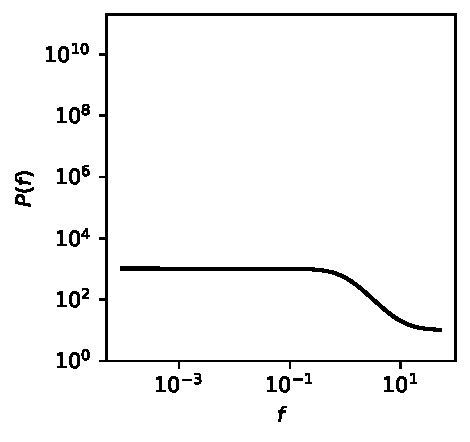
\includegraphics[width=0.3\textwidth]{0.1/small_condition_num/P_f.pdf}
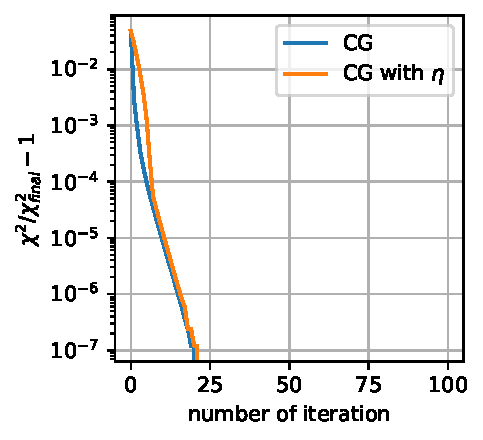
\includegraphics[width=0.3\textwidth]{0.1/small_condition_num/chi2_CG.pdf}
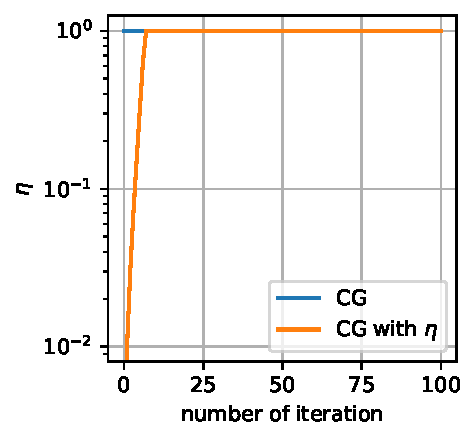
\includegraphics[width=0.3\textwidth]{0.1/small_condition_num/eta_CG.pdf}
\caption{The left graph shows the noise power spectrum
    Eq.(\ref{noise power spectrum}) with $f_{\text{apo}} \approx 0.99$ and
    $\kappa(N) = 10^2$. The center one shows the
    $\chi^2(\vbm)/\chi^2_{\text{final}} - 1$, with $\chi^2(\vbm)$ calculated
    based on Eq.(\ref{chi2 formula}).
    The right one shows the $\eta$ value for each iteration. For vanilla 
    conjugate gradient method $\eta$ always equal to $1$, so it's a horizontal
    line at $\eta=1$.
}
\label{small condi num CG}
\end{figure*}

Notice that as we increase $\kappa(N)$, or equivalently decrease
$f_{\text{apo}}$, the perturbation parameter $\eta$ starts showing its 
benefits, as showed in Figure(\ref{medium condi num CG}) and 
Figure(\ref{large condi num CG}).
It outperforms the vanilla conjugate gradient method when 
$f_{\text{apo}} \approx 0$ and the noise power spectrum becomes the $1/f$ noise model,
which usually is the intrinsic noise of instruments (\cite{1997PhRvD..56.4514T}).
\begin{figure*}[htb!]
\centering
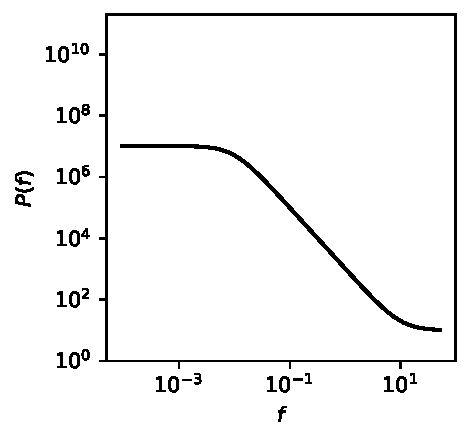
\includegraphics[width=0.3\textwidth]{0.1/medium_condition_num/P_f.pdf}
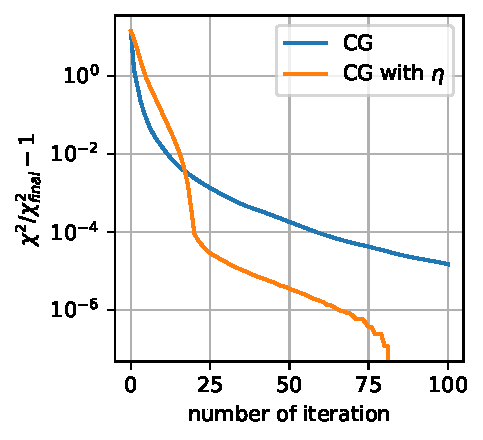
\includegraphics[width=0.3\textwidth]{0.1/medium_condition_num/chi2_CG.pdf}
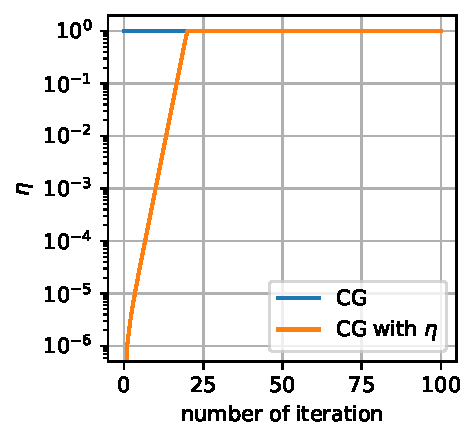
\includegraphics[width=0.3\textwidth]{0.1/medium_condition_num/eta_CG.pdf}
\caption{The figure shows results for $f_{\text{apo}}\approx 9.8\times10^{-3}$ 
    and $\kappa(N) = 10^6$.
}
\label{medium condi num CG}
\end{figure*}

\begin{figure*}[htb!]
\centering
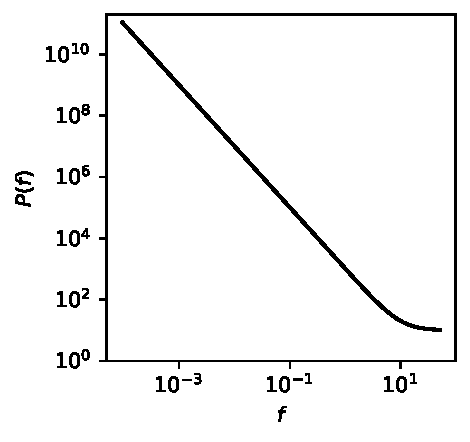
\includegraphics[width=0.3\textwidth]{0.1/large_condition_num/P_f.pdf}
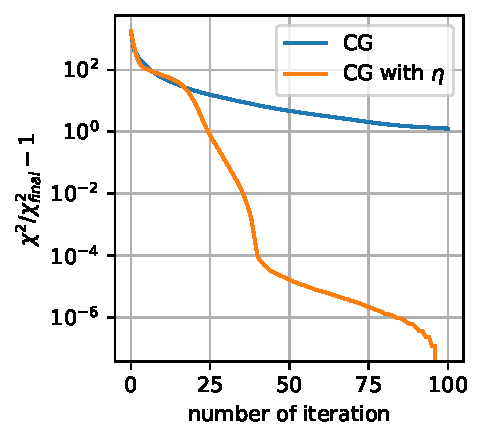
\includegraphics[width=0.3\textwidth]{0.1/large_condition_num/chi2_CG.pdf}
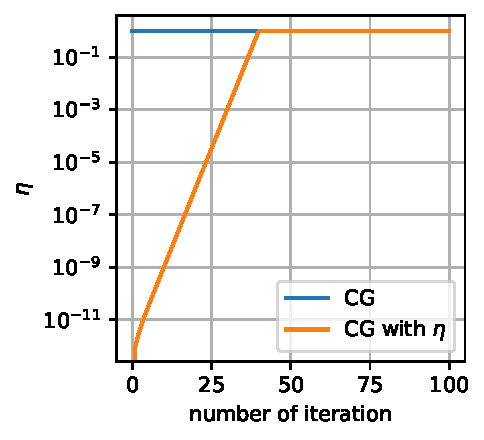
\includegraphics[width=0.3\textwidth]{0.1/large_condition_num/eta_CG.pdf}
\caption{The figure shows results for $f_{\text{apo}}\approx 9.8\times10^{-6}$ 
    and $\kappa(N) = 10^{12}$.
}
\label{large condi num CG}
\end{figure*}

%In the conjugate gradient method with messenger cooling parameter $\lambda$, 
%the number of cooling parameters we need is an extra free parameter.
%After the number of $\lambda$ is determined, we construct a geometric series
%with fixed initial and final value, which uses \texttt{logspace}
%function in \texttt{numpy}.
%Since I  show in Eq.(\ref{lambda eta equiv}) that the messenger field
%cooling parameter $\lambda$ is equivalent to $1/\eta$, I use $\eta$ for further analysis.

Now let us compare the performance difference between choosing $\eta$
parameters based on Eq.(\ref{etai rule})
and manually fixing number of $\eta$ parameters $n_{\eta}$ manually.
We manually choose the $\eta_i$ values using function
\texttt{numpy.logspace(start=$\ln(\eta_1)$, stop=0, num=$n_{\eta}$, base=$e$)}.
The results are showed in Figure(\ref{small condi num}),
(\ref{medium condi num}), and (\ref{large condi num}).

When $\kappa(N)$ is small, and Eq.(\ref{etai rule}) tells us that only a few
$\eta$ parameters are good enough, see the orange line in the last Figure(\ref{small condi num}).
If unfortunately we choose $n_{\eta}$ being large value, like $15$ or $30$,
then it will ends up converge slowly, because it needs at least $15$ or $30$
iterations to reach $\eta=1$, at least one iteration per $\eta$ level.

On the other hand if $\kappa(N)$ is very large and the power spectrum is $1/f$
noise, we need more $\eta$ parameters.
If $n_{\eta}$ is too small, for example $n_{\eta}=5$ the red line in
Figure(\ref{large condi num}), it may be better than the vanilla conjugate
gradient method, but it is still far from optimal.


\begin{figure*}[htb!]
\centering
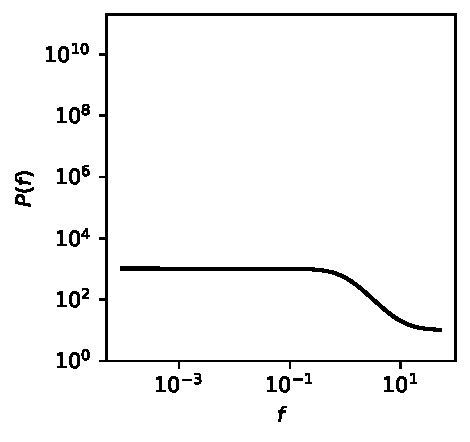
\includegraphics[width=0.3\textwidth]{0.1/small_condition_num/P_f.pdf}
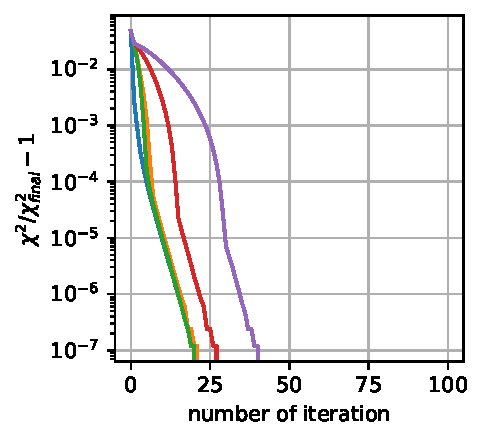
\includegraphics[width=0.3\textwidth]{0.1/small_condition_num/chi2.pdf}
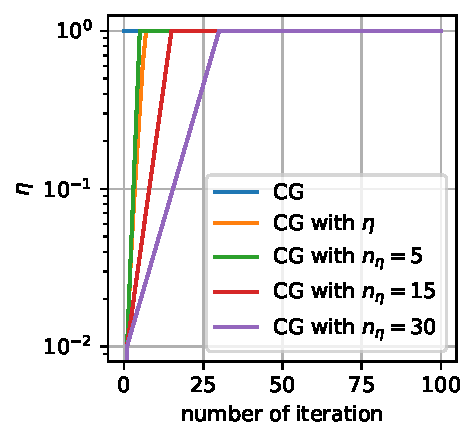
\includegraphics[width=0.3\textwidth]{0.1/small_condition_num/eta.pdf}
\caption{Same as Figure(\ref{small condi num CG}) with extra manually chosen 
    $n_{\eta}$ results.
}
\label{small condi num}
\end{figure*}


\begin{figure*}[htb!]
\centering
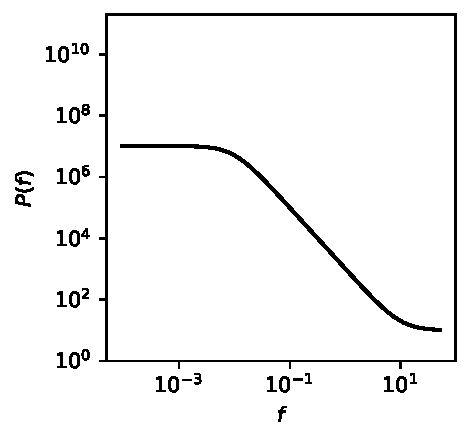
\includegraphics[width=0.3\textwidth]{0.1/medium_condition_num/P_f.pdf}
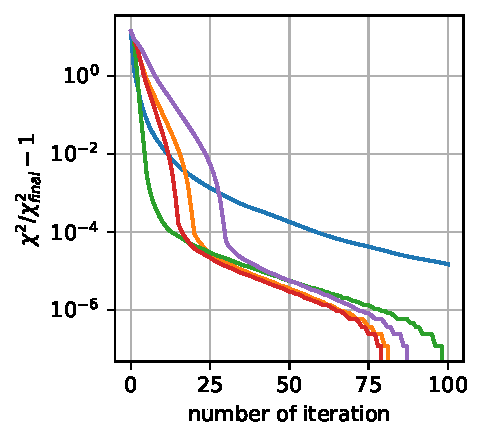
\includegraphics[width=0.3\textwidth]{0.1/medium_condition_num/chi2.pdf}
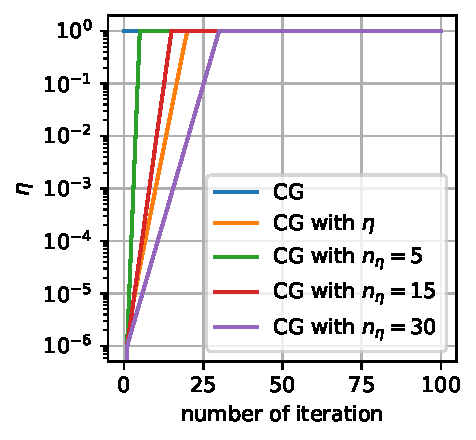
\includegraphics[width=0.3\textwidth]{0.1/medium_condition_num/eta.pdf}
\caption{Same as Figure(\ref{medium condi num CG}) with extra manually chosen 
    $n_{\eta}$ results.
}
\label{medium condi num}
\end{figure*}

\begin{figure*}[htb!]
\centering
\includegraphics[width=0.3\textwidth]{0.1/large_condition_num/p_f.pdf}
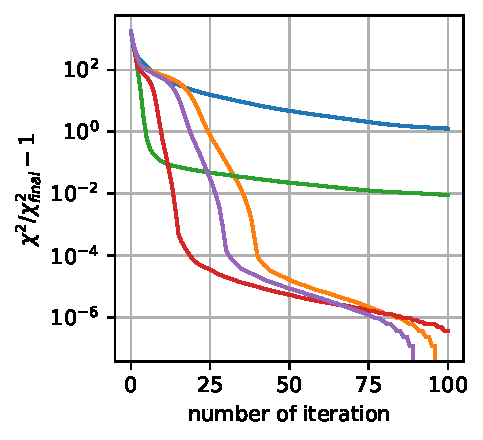
\includegraphics[width=0.3\textwidth]{0.1/large_condition_num/chi2.pdf}
\includegraphics[width=0.3\textwidth]{0.1/large_condition_num/eta.pdf}
\caption{Same as Figure(\ref{large condi num CG}) with extra manually chosen 
    $n_{\eta}$ results.
}
\label{large condi num}
\end{figure*}

\section{Future Prospects and Conclusion}
As you may have noticed in Figure(\ref{medium condi num})
and Figure(\ref{large condi num}), the perturbation parameter based on
Eq.(\ref{etai rule}) is more than needed, especially for $1/f$ noise case.
From the last graph in Figure(\ref{large condi num}) we notice that
Eq.(\ref{etai rule}) gives us $n_{\eta}\approx40$, however based on $\chi^2$
result in Figure(\ref{large condi num}) 
$n_{\eta}\approx30$ or even $n_{\eta} \approx 15$ is good enough.
Also, for the nearly-white-noise case, we could certainly choose $n_{\eta}=1$
such that $\eta_1=1$ which corresponds to vanilla conjugate gradient method,
based on $\chi^2$ result in Figure(\ref{small condi num}).
However Eq.(\ref{etai rule}) gives us $n_{\eta} \approx 6$,
see the last last graph in Figure(\ref{small condi num}),
even though it does not make the final $\chi^2$ result much different at the
end.

Is it possible to further improve the analysis, such that it produces
smaller $n_{\eta}$?
Let's examine how we get $\eta_i$ series.
Remember that we determine $\delta\eta$ value based on the upper bound of 
$-\delta\chi^2(\hatm(\eta), \eta)/\chi^2(\hatm(\eta), \eta)$, in
Eq.(\ref{eta upper bound}).
For $\eta \neq 0$, the upper bound is
%Here I rewrite it in a simplified form
\begin{align}
%-\frac{\delta\chi^2(\hatm(\eta), \eta)}{\chi^2(\hatm(\eta), \eta)}
%%= -\delta\eta
%%    \frac{\dv{\eta} \chi^2(\hatm(\eta), \eta)}
%%    {\chi^2(\hatm(\eta), \eta)}
\delta\eta \frac{\hat{\vb{r}}_{\eta}^{\dagger} \inv{N(\eta)} \Nbar 
    \inv{N(\eta)} \hat{\vb{r}}_{\eta} }
    {\hat{\vb{r}}_{\eta}^{\dagger} \inv{N(\eta)} \hat{\vb{r}}_{\eta} }
%\\
\leq  \frac{\delta \eta}{\eta + \frac{\tau}{\max(N_f) -\tau}}
\end{align}
with
$
\vb{r}_{\eta} %= \vbd - P\hatm(\eta) 
= \qty[ 1 - P\PPinv{\inv{N(\eta)}}\Pdagger \inv{N(\eta)}]\vbd
\equiv \mathcal{P}_{\eta} \vbd
$.
To get the upper bound we treated $\vbd - P\hatm(\eta)$ as an arbitrary 
vector in frequency domain, since we don't know how to calculate 
$\mathcal{P}_{\eta}$ for $\eta \neq 0$, and it's hard to 
analyze the projection matrix $\mathcal{P}_{\eta}$ in frequency space,
as it contains $\PPinv{\inv{N(\eta)}}$.
Note that we have to determine all of $\eta$ value before calculation, 
because we don't want to keep the time ordered data in system RAM,
so we need to somehow analytically analyze $\mathcal{P}_{\eta}$, and its behavior
in frequency space.
Unless $\vb{r}_{\eta}$ almost only has large noise modes,
$\qty|\dv{\eta}\chi^2(\hatm(\eta),\eta)/\chi^2(\hatm(\eta),\eta)|$
won't get close to the upper bound
$1/\qty(\eta + \frac{\tau}{\max(N_f) -\tau})$.
Based on the analysis in Section(\ref{intuitive interp}),
for small $\eta$ the estimated map $\hatm(\eta)$ does not only focusing on 
minimizing error $\vb{r}_{\eta}$ at low noise region.
So we would expect that there would be a fair amount of low noise modes
contribution in $\vb{r}_{\eta}$ especially for the first few $\eta$ values.
Which means if we could somehow know the frequency distribution of 
$\vb{r}_{\eta}$, we could tighten the boundary of
$\qty|\dv{\eta}\chi^2(\hatm(\eta),\eta)/\chi^2(\hatm(\eta),\eta)|$,
and get larger $\delta\eta$ value.
This should make $\eta$ goes to $1$ faster, and yields the fewer $\eta$ parameters 
we need.

Also notice that the $\eta$ values determined from Eq.(\ref{etai rule})
%\begin{align}
%\eta_i =\min \qty\bigg{1,\; \frac{\tau}{\max(\Nbar_f)} \qty(2^i -1) } 
%\tag{\ref{etai rule}}
%\end{align}
are not dependent on any scanning information,
it only depends on noise power spectrum $P(f)$, or noise covariance matrix $N$.
In Appendix \ref{other cases} we would show 
%Figure(\ref{large condi num 0.001}) and Figure(\ref{large condi num 10}) show
two examples with same parameters as in Figure(\ref{large condi num}) except 
scanning frequency $f_{\text{scan}}$.%, in Figure(\ref{large condi num 0.001}) it
%scans very slow and in Figure(\ref{large condi num 10}) it's very fast.
%In these two cases our $\eta$ values based on Eq.(\ref{etai rule}) are better
%than manually selected values.
%Based on these two results we know,
It turns out the $\eta$ values should somehow depends
on scanning scheme.
Again that's because when we determine the upper bound% of 
%$\dv{\eta} \chi^2(\hatm(\eta), \eta)$
we treated
$\vb{r}_{\eta}$ % = \vbd - P\hatm = \mathcal{P}_{\eta} \vbd$
as an arbitrary vector, such that we lose all information related to scanning 
scheme in the pointing matrix $P$.


%\begin{figure*}[htb!]
%\centering
%\includegraphics[width=0.3\textwidth]{0.001/large_condition_num/p_f.pdf}
%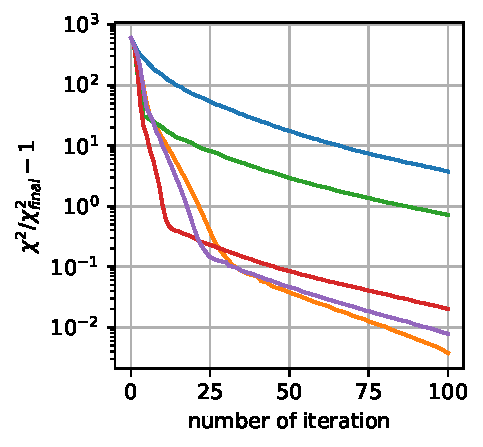
\includegraphics[width=0.3\textwidth]{0.001/large_condition_num/chi2.pdf}
%\includegraphics[width=0.3\textwidth]{0.001/large_condition_num/eta.pdf}
%\caption{In this case all frequencies are the same as
%    Figure(\ref{large condi num}) except $f_{\text{scan}} = 0.001$.
%}
%\label{large condi num 0.001}
%\end{figure*}
%
%\begin{figure*}[htb!]
%\includegraphics[width=0.3\textwidth]{10/large_condition_num/p_f.pdf}
%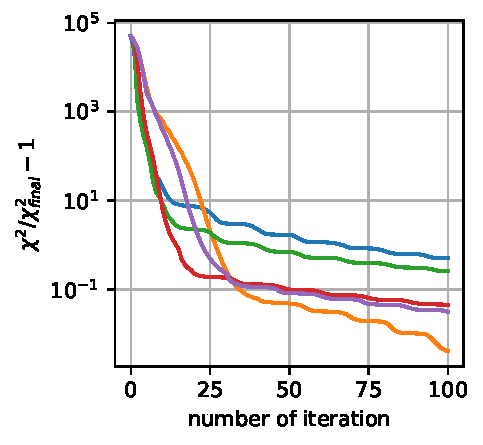
\includegraphics[width=0.3\textwidth]{10/large_condition_num/chi2.pdf}
%\includegraphics[width=0.3\textwidth]{10/large_condition_num/eta.pdf}
%\caption{In this case all frequencies are the same as
%    Figure(\ref{large condi num}) except $f_{\text{scan}} = 10$.
%}
%\label{large condi num 10}
%\end{figure*}



%\section{Conclusion}
%Here we discussed a method to solve map making equation
%Eq.(\ref{map making equation})
%\begin{align}
%\hatm = \PPinv{N} \Pdagger \inv{N} \vbd \tag{\ref{map making equation}}
%\end{align}
%by separating noise covariance matrix $N$ into two parts, white noise part
%$\tau I$ and the remaining noise $\Nbar$.
%Then we could think $\Nbar$ as a perturbation added to white noise, 
%by introducing a parameter $\eta$, as $\eta$ change from $0$ to $1$,
%we gradually add this non white noise in to system.
%
%The $\eta$ values can be predetermined analytically.
%This property is very important, because we don't want to keep entire time
%ordered data in system RAM.
%If these $\eta$ values can be determined before calculation, then we only need
%to keep several map sized object, which is much smaller than timed ordered 
%data.
%Also we showed that this method has same computational cost as vanilla
%conjugate gradient method but performs better when the condition number of 
%noise covariance matrix $\kappa(N)$ is large, especially in $1/f$ noise case.
%The only extra free parameter added is to determine whether the error at
%current step $\vb{r}(\eta_i) = \qty||\vbb(\eta_i) - A(\eta_i) \vbm||$ is small
%enough such that we change advance to next value $\eta_{i+1}$.

Even though the perturbation parameter $\eta$ get from Eq.(\ref{etai rule}) are
not the most optimal,
it still performs much better than traditional conjugate gradient method under
$1/f$ noise scenario without adding extra computational cost.
The only extra free parameter added is to determine whether the error at
current step $\vb{r}(\eta_i) = \qty||\vbb(\eta_i) - A(\eta_i) \vbm||$ is small
enough such that we advance to next value $\eta_{i+1}$.
%Since it only takes in to account the noise information in $N$,
%but ignored all scanning information contained in pointing matrix $P$, because
%we are unable to analyze the structure of
%$\vb{r}_{\eta} = \vbd - P\hatm(\eta) = \mathcal{P}_{\eta} \vbd$ in frequency
%space.


Also this analysis of $\eta$ value also explains why cooling parameters
$\lambda=1/\eta$ in messenger field are chosen to be geometric series or
\texttt{logspace} used in \cite{Huffenberger_2018}.

All of the calculation are using simple preconditioner $\Pdagger P$, but 
the entire analysis is independent of preconditioner.
Using better preconditioners, it would also have improvements.















%% IMPORTANT! The old "\acknowledgment" command has be depreciated. It was
%% not robust enough to handle our new dual anonymous review requirements and
%% thus been replaced with the acknowledgment environment. If you try to 
%% compile with \acknowledgment you will get an error print to the screen
%% and in the compiled pdf.
%\begin{acknowledgments}
%\end{acknowledgments}

%% To help institutions obtain information on the effectiveness of their 
%% telescopes the AAS Journals has created a group of keywords for telescope 
%% facilities.
%
%% Following the acknowledgments section, use the following syntax and the
%% \facility{} or \facilities{} macros to list the keywords of facilities used 
%% in the research for the paper.  Each keyword is check against the master 
%% list during copy editing.  Individual instruments can be provided in 
%% parentheses, after the keyword, but they are not verified.

%\vspace{5mm}
%\facilities{HST(STIS), Swift(XRT and UVOT), AAVSO, CTIO:1.3m,
%CTIO:1.5m,CXO}

%% Similar to \facility{}, there is the optional \software command to allow 
%% authors a place to specify which programs were used during the creation of 
%% the manuscript. Authors should list each code and include either a
%% citation or url to the code inside ()s when available.

%\software{astropy \citep{2013A&A...558A..33A,2018AJ....156..123A},  
%          Cloudy \citep{2013RMxAA..49..137F}, 
%          Source Extractor \citep{1996A&AS..117..393B}
%          }

%% Appendix material should be preceded with a single \appendix command.
%% There should be a \section command for each appendix. Mark appendix
%% subsections with the same markup you use in the main body of the paper.

%% Each Appendix (indicated with \section) will be lettered A, B, C, etc.
%% The equation counter will reset when it encounters the \appendix
%% command and will number appendix equations (A1), (A2), etc. The
%% Figure and Table counter will not reset.

\vspace{5mm}
\appendix

\section{Upper bound for $\eta$} \label{derive other etas}
We want to find the upper bound for 
$
-\frac{\delta \chi^2(\hatm(\eta_m),\eta_m)} {\chi^2(\hatm(\eta_m), \eta_m)}
$
First let's calculate $\dv{\eta} \chi^2(\hatm(\eta), \eta)$
\begin{align}
\begin{aligned}[b]
\dv{\eta} \chi^2(\hatm(\eta), \eta)  &= \pdv{\eta} \chi^2(\hatm(\eta), \eta) \\
&= \pdv{\eta} \qty\big(\vbd - P \hatm(\eta))^{\dagger} \inv{N(\eta)} 
    \qty\big(\vbd - P\hatm(\eta))\\
&= - \qty(\vbd - P\hatm(\eta))^{\dagger} \inv{N(\eta)} \Nbar \inv{N(\eta)} 
    (\vbd - P\hatm(\eta))\\
&= - \vb{r}^{\dagger}(\eta) \inv{N(\eta)} \Nbar \inv{N(\eta)} \vb{r}(\eta)
\label{d chi2}.
\end{aligned}
\end{align}
where the first line comes from, $\chi^2(\hatm(\eta),\eta)$ is minimum $\chi^2$
value for certain $\eta$, therefore $\pdv{\vbm} \chi^2(\vbm, \eta) \Bigr|_{\vbm = \hatm(\eta)} = 0$.
So the third line we only take partial derivative with respect to $\inv{N(\eta)}$.
The last line we define $\vb{r}(\eta) =\vbd - P\hatm(\eta)$.

The upper bound is given by
\begin{align}
\begin{aligned}[b]
-\frac{\delta \chi^2(\hatm(\eta_m), \eta_m)}{\chi^2(\hatm(\eta_m), \eta_m)}  
&= \delta\eta_m
\frac{\vb{r}^{\dagger}
    \inv{N(\eta_m)} \Nbar \inv{N(\eta_m)}
    \vb{r}
}
{ \vb{r}^{\dagger}
    \inv{N(\eta_m)}
    \vb{r}
}
\\
& \leq \delta \eta_m\, \max\qty(\frac{\Nbar_f}{\tau + \eta_m \Nbar_f})
%\label{eta upper bound}
\end{aligned}
\end{align}

For the last line, both matrix $\Nbar$ and $\inv{N(\eta_m)}$ 
can be simultaneously diagonalized in frequency space.
For each eigenvector $\vb{e}_f$,
the corresponding eigenvalues of the matrix 
$\inv{N(\eta_m)} \Nbar \inv{N(\eta_m)}$
are
$\lambda_f = \Nbar_f (\tau + \eta_m \Nbar_f)^{-2}$,
and the eigenvalues for matrix 
$\inv{N(\eta_m)}$
are
$\gamma_f = (\tau + \eta_m \Nbar_f)^{-1}$.
Their eigenvalues are related by
$\lambda_f = \frac{\Nbar_f}{\tau + \eta_m \Nbar_f} \gamma_f$.
For vector $\vb{r} = \sum_f \alpha_f \vb{e}_f$, we have
$\frac{\vb{r}^{\dagger} \inv{N(\eta_m)} \Nbar \inv{N(\eta_m)} \vb{r}}
{\vb{r}^{\dagger} \inv{N(\eta_m)} \vb{r}}
= \frac{\sum_f \alpha_f^2 \lambda_f}{\sum_f \alpha_f^2 \gamma_f}
= \frac{\sum_f \alpha_f^2 \gamma_f \Nbar_f/(\tau + \eta_m \Nbar_f)}
{\sum_f \alpha_f^2 \gamma_f}
\leq \max \qty( \frac{\Nbar_f}{\tau + \eta_m \Nbar_f})
$.

If we set the upper bound
$\delta\eta_m \max \qty( \frac{\Nbar_f}{\tau + \eta_m \Nbar_f})=1$,
\footnote{Here we also assumed that
$\chi^2(\hatm(\eta_m),\eta_m) \gg \chi^2(\hatm(1),1)$,
which we expect it to be satisfied for $0 \simeq \eta_m \ll 1$. 
Since final result Eq.(\ref{etai rule}) is geometric series,
only a few $\eta_m$ values won't satisfy this condition.
}
and then we get
\begin{align}
\delta \eta_m 
= \min \qty(\frac{\tau + \eta_m \Nbar_f}{\Nbar_f})
= \eta_m + \frac{\tau }{\max(\Nbar_f)}.
\end{align}

\vspace{5mm}
\section{Other Cases} \label{other cases}

%Here we show two other results with different scaning frequency from Figure.(\ref{large condi num}),
%but keep every other parameters sames.
Since the $\eta$ values determined from Eq.(\ref{etai rule})
\begin{align}
\eta_i =\min \qty\bigg{1,\; \frac{\tau}{\max(\Nbar_f)} \qty(2^i -1) } 
\tag{\ref{etai rule}}
\end{align}
are not dependent on any scanning information,
it only depends on noise power spectrum $P(f)$, or noise covariance matrix $N$.
Figure(\ref{large condi num 0.001}) and Figure(\ref{large condi num 10}) show
two examples with same parameters as in Figure(\ref{large condi num}) except 
scanning frequency $f_{\text{scan}}$, in Figure(\ref{large condi num 0.001}) it
scans very slow and in Figure(\ref{large condi num 10}) it's very fast.
In these two cases our $\eta$ values based on Eq.(\ref{etai rule}) are better
than manually selected values.
Based on these two results we know, the $\eta$ values should somehow depends
on scanning scheme.

\begin{figure*}[htb!]
\centering
\includegraphics[width=0.3\textwidth]{0.001/large_condition_num/p_f.pdf}
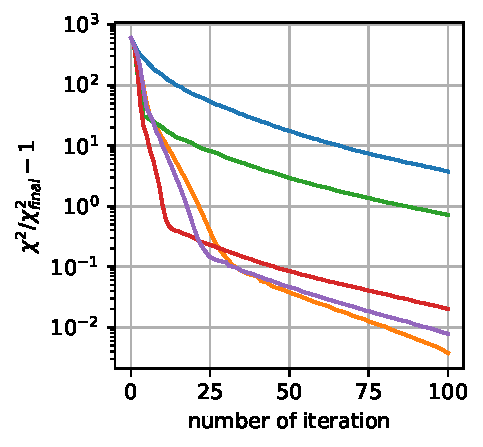
\includegraphics[width=0.3\textwidth]{0.001/large_condition_num/chi2.pdf}
\includegraphics[width=0.3\textwidth]{0.001/large_condition_num/eta.pdf}
\caption{In this case all frequencies are the same as
    Figure(\ref{large condi num}) except $f_{\text{scan}} = 0.001$.
}
\label{large condi num 0.001}
\end{figure*}

\begin{figure*}[htb!]
\includegraphics[width=0.3\textwidth]{10/large_condition_num/p_f.pdf}
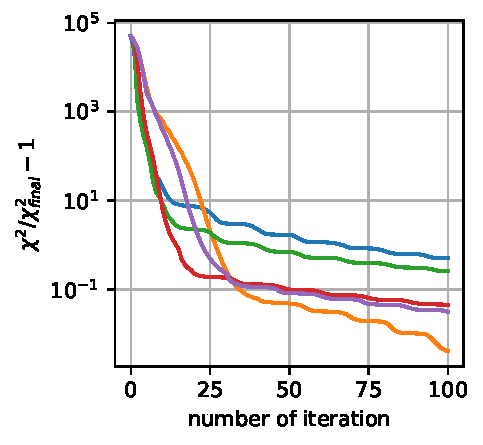
\includegraphics[width=0.3\textwidth]{10/large_condition_num/chi2.pdf}
\includegraphics[width=0.3\textwidth]{10/large_condition_num/eta.pdf}
\caption{In this case all frequencies are the same as
    Figure(\ref{large condi num}) except $f_{\text{scan}} = 10$.
}
\label{large condi num 10}
\end{figure*}









%% For this sample we use BibTeX plus aasjournals.bst to generate the
%% the bibliography. The sample631.bib file was populated from ADS. To
%% get the citations to show in the compiled file do the following:
%%
%% pdflatex sample631.tex
%% bibtext sample631
%% pdflatex sample631.tex
%% pdflatex sample631.tex

\bibliography{references.bib}{}
\bibliographystyle{aasjournal}

%% This command is needed to show the entire author+affiliation list when
%% the collaboration and author truncation commands are used.  It has to
%% go at the end of the manuscript.
%\allauthors

%% Include this line if you are using the \added, \replaced, \deleted
%% commands to see a summary list of all changes at the end of the article.
%\listofchanges

\end{document}

% End of file `sample631.tex'.
